\documentclass{article}
\usepackage{graphicx}
\usepackage[export]{adjustbox}
\usepackage{tabularx}  %better tables
\usepackage{hyperref}

\title{Homework 4 CSCI 451}
\author{Nicholas Rust}
\date{due: 05 November 2019}

\begin{document}
\maketitle

\section{Exercise 2 (textbook section 6.9, pg 152)}

Scoring:\\
Mismatch = 1\\
Gap = 2

\noindent\rule{8cm}{0.4pt}

\begin{verbatim} 
ACTCTCGATC 
ACT-TCGATC
\end{verbatim}
Mismatch: 0\\
Gap: 1\\
Distance from $S_1$ to $S_2$ is 2.

\noindent\rule{8cm}{0.4pt}

\begin{verbatim} 
ACTCTCGATC 
ACTCTCTATC
\end{verbatim}
Mismatch: 1\\
Gap: 0\\
Distance from $S_1$ to $S_3$ is 1.

\noindent\rule{8cm}{0.4pt}

\begin{verbatim} 
ACTCTCGA-TC 
ACTCTCTAATC
\end{verbatim}
Mismatch: 1\\
Gap: 1\\
Distance from $S_1$ to $S_4$ is 3.

\noindent\rule{8cm}{0.4pt}

\begin{verbatim} 
ACT-TCGATC 
ACTCTCTATC
\end{verbatim}
Mismatch: 1\\
Gap: 1\\
Distance from $S_2$ to $S_3$ is 3.

\noindent\rule{8cm}{0.4pt}

\begin{verbatim} 
ACT-TC-GATC 
ACTCTCTAATC
\end{verbatim}
Mismatch: 1\\
Gap: 2\\
Distance from $S_2$ to $S_4$ is 5.

\noindent\rule{8cm}{0.4pt}

\begin{verbatim} 
ACTCTCT-ATC 
ACTCTCTAATC
\end{verbatim}
Mismatch: 0\\
Gap: 1\\
Distance from $S_3$ to $S_4$ is 2.

\noindent\rule{8cm}{0.4pt}

Summation of distances for each string:\\
$S_1:6$\\
$S_2:10$\\
$S_3:6$\\
$S_4:10$\\

Therefore either $S_1$ or $S_3$ is the center string, here we use $S_1$.
\begin{verbatim} 
ACTCTCGA-TC
ACT-TCGA-TC
ACTCTCTA-TC
ACTCTCTAATC
\end{verbatim}

Notice when aligning the fourth string we have to put a gap in every preceding string as well as the center.

\section{Exercise 3 (textbook section 6.9, pg 152)}
\textbf{Step 1:} Compute optimal global alignment for each pair of strings.
I did this above for center star.\\
\textbf{Step 2:} Use $1-y/x$ to compute the distance matrix. 

\vspace{.5cm}

\bgroup
\def\arraystretch{1.5}%
\begin{tabularx}{8cm}{| X | X | X | X | X |}
  \hline
  \textbf{~} & \textbf{$S_1$} & \textbf{$S_2$} & \textbf{$S_3$} & \textbf{$S_4$}\\
  \hline	
  \textbf{$S_1$} & 0 & 0 & .1 & .1		\\
  \textbf{$S_2$} & ~ & 0 & .111 & .111	\\
  \textbf{$S_3$} & ~ & ~ & 0 & 0		\\
  \textbf{$S_4$} & ~ & ~ & ~ & 0		\\ 
  \hline
\end{tabularx}
\egroup

\vspace{.5cm}

\textbf{Step 3:} Compute the guide tree using neighbor joining magic. The order in which they are joined will be $S_1$, $S_3$, $S_2$, $S_4$.

\textbf{Step 4:} Follow the tree bottom-up to find the correct alignments, which will look something like:
\begin{verbatim} 
ACTCTCG-ATC
ACT-TCG-ATC
ACTCTCT-ATC
ACTCTCTAATC
\end{verbatim}

\section{Exercise 4 (textbook section 6.9, pg 152)}
Something similar to center star could be effective. Center star does a global alignment of the strings, if we wanted to find local alignments that maximize the score we could find a center string on the global level. We then do a pairwise local match with this string($S_c$) and another($S_2$), but take whatever subset of $S_2$ provides us with the most maximized score. We can then search for similar substrings of strings $S_3,...,S_k$ using the z-algorithm (with room for a number of differences). This will give us a semi-decent guess of the most optimized local alignments. It won't be the fastest algorithm since we still have the O($n^2k^2$) time complexity to find the distances between each string which will be the most significant time complexity.

\newpage
\begin{figure}
	\section{Programming project: Center Sequence Finder}
    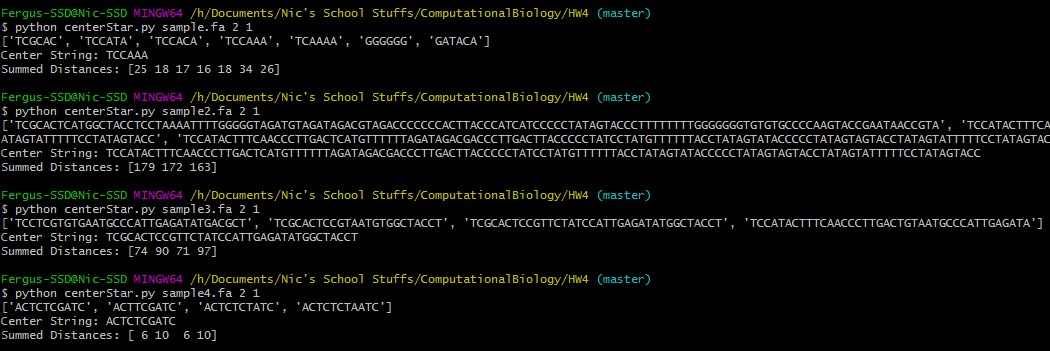
\includegraphics[width=1.75\textwidth,center]{HW4output.jpg}
    \caption{Program Output}
\end{figure}


\end{document}